\vspace{+15pt}
\section{Auswertung}
\label{sec:Auswertung}

\vspace{+15pt}
\subsection{Vorbereitende Berechnungen}
\vspace{+5pt}

Der erste Detektorscan wird mittels Funktion 
\textit{scipy.optimize.curve\_fit} aus der Python-Bibliothek SkiPy nach der Gaußfunktion

\begin{equation}
    f(\alpha_i) = \frac{a}{\sqrt{2 \pi \sigma^2}} \text{exp}\left(- \frac{(\alpha_i - \mu)^2}{2\sigma^2}\right) + b
\end{equation}

\vspace{+10pt}
approximiert und ist in Abbildung \ref{fig:plot1} dargestellt.
Die Näherungsparameter ergeben sich zu
\vspace{-25pt}

\begin{align*}
    \mu &= (\num{-4.1 +- 0.5}) \cdot 10^{-3}\si{\degree} \; ,\\
    \sigma &= (\num{45.9 +- 0.6}) \cdot 10^{-3} \si{\degree} \; ,\\
    a &= (\num{18.55 +- 0.22}) \cdot 10^4 \; ,\\
    b &= (\num{1.6 +- 0.4}) \cdot 10^4 \; .
\end{align*}

\vspace{-7pt}
\begin{figure}[H]
    \centering
    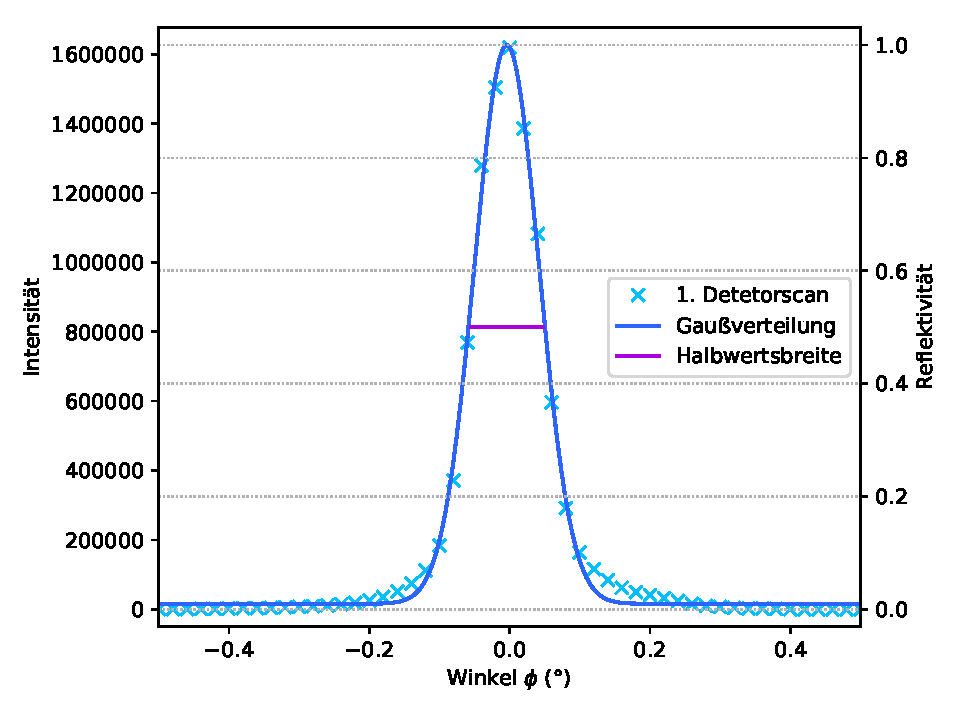
\includegraphics[scale=0.7]{content/plot1.pdf}
    \vspace{-10pt}
    \caption{Gaußgenäherte Intensität des ersten Detektorscans in Abhängigkeit des Einfallswinkels $\alpha_i$.}
    \label{fig:plot1}
\end{figure}

Aus den aufgenommenen Daten und des Maximums der Gaußnäherung ergeben sich die maximalen
Intensitäten von 
\vspace{-25pt}

\begin{align*}
    I_\text{max,detec} &= \num{1618610} \; ,\\
    I_\text{max,gauss} &= \num{1626579.26}
\end{align*}

und die Halbwertsbreite der Näherung von

\begin{equation*}
    d_{\sfrac{1}{2}} = \SI{0.12}{\degree} \; .
\end{equation*}

In Abbildung \ref{fig:plot21} ist der erste Z-Scan dargestellt.
Aus diesem lässt sich anhand der Differenz der Höhen rechts und links der negativen Flanke der Intensität
die Strahldicke als etwa

\begin{equation*}
    d_0 = \SI{0.28}{\milli\meter}
\end{equation*}

bestimmen. Zudem übersteigt hier die maximale Intensität die des Detektorscans mit 

\begin{equation}
    I_\text{max,z} = \num{1636650} \; ,
    \label{eqn:imax}
\end{equation}

mit welcher die Reflektivitäten der folgenden Scans normiert werden sollen.

\begin{figure}[H]
    \centering
    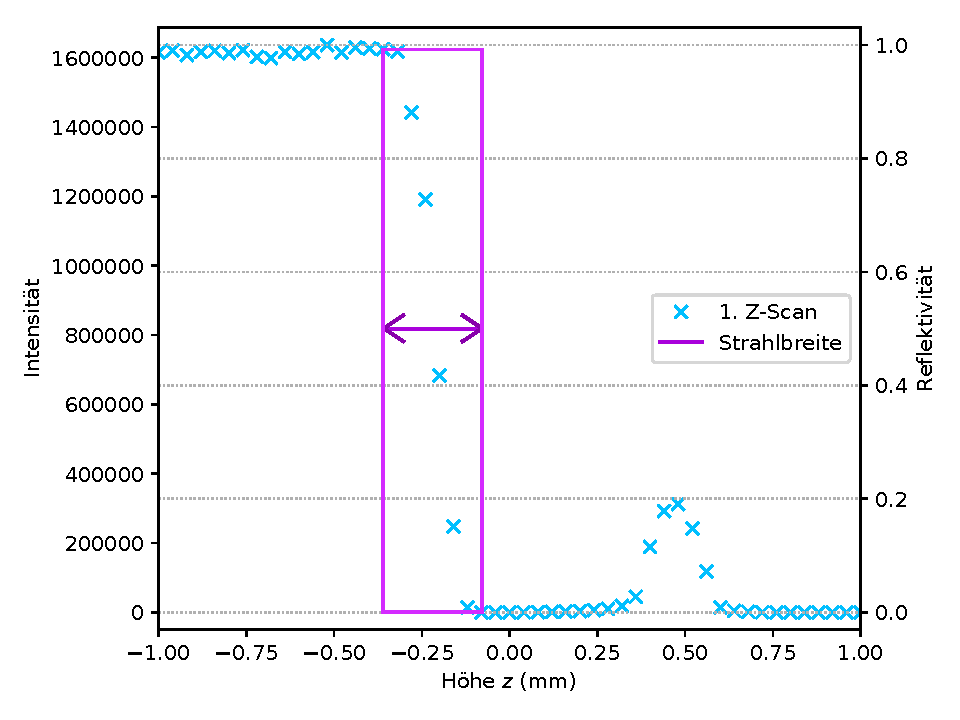
\includegraphics[scale=0.7]{content/plot21.pdf}
    \vspace{-10pt}
    \caption{Intensität des Z-Scans in Abhängigkeit der Probenhöhe $z$.}
    \label{fig:plot21}
\end{figure}

Aus dem in Abbildung \ref{fig:plot21} dargestellten ersten Rockingscans
können links und rechts des Intensitätspeaks die beiden Geometriewinkel $\alpha_{g,i}$
abgelesen werden, deren Intensitäten gerade nicht verschwindend sind. 
Zusammen mit dem gemitteltem Winkel $\alpha_g$ ergeben sich diese zu

\vspace{-25pt}
\begin{align*}
    \alpha_{g,1} &= \SI{-0.84}{\degree} \; , \\
    \alpha_{g,2} &= \SI{0.64}{\degree} \; , \\
    \alpha_{g} = \sfrac{1}{2}|\alpha_{g,1} &- \alpha_{g,2}| = \SI{0.74}{\degree} \; .
\end{align*}

Alternativ kann der Geometriewinkel auch über Strahlbreite $d_0 = \SI{0.28}{\milli\meter}$ und 
die Probendicke $D = \SI{20}{\milli\meter}$ bestimmt werden zu

\begin{equation}
    \alpha'_g = \text{arcsin} \left(\sfrac{d_0}{D}\right) \approx \SI{0.8}{\degree}  \; .
\end{equation}


\section{Scananwendung zur Vermessung eines mit Polystyrol beschichteten Silizium-Wafers}

Für die eigentliche Messung wurden ein Reflektivitäts- und ein Diffuser Scan angewandt und deren Daten aufbereitet,
sodass sich die in Abbildung \ref{fig:plot4} dargestellten Ergebnisse zeigen.
Zur Bestimmung der Reflektivitäten werden die Intensitäten auf die fünffache maximale Intensität des 
Z-Scans \eqref{eqn:imax} normiert. Damit wird berücksichtigt, dass die Messdauer im Vergleich zu den Justagemessungen
von $\SI{1}{\second}$ auf $\SI{5}{\second}$ erhöht wurde.
Weiterhin werden die Daten statt in Winkelabhängigkeit, in Abhängigkeit des Wellenvektorübertrags 
$q = \frac{4\pi}{\lambda} \cdot \text{sin} \left(\frac{\pi}{180}\alpha_i\right)$ dargestellt.\\

\begin{figure}[H]
    \centering
    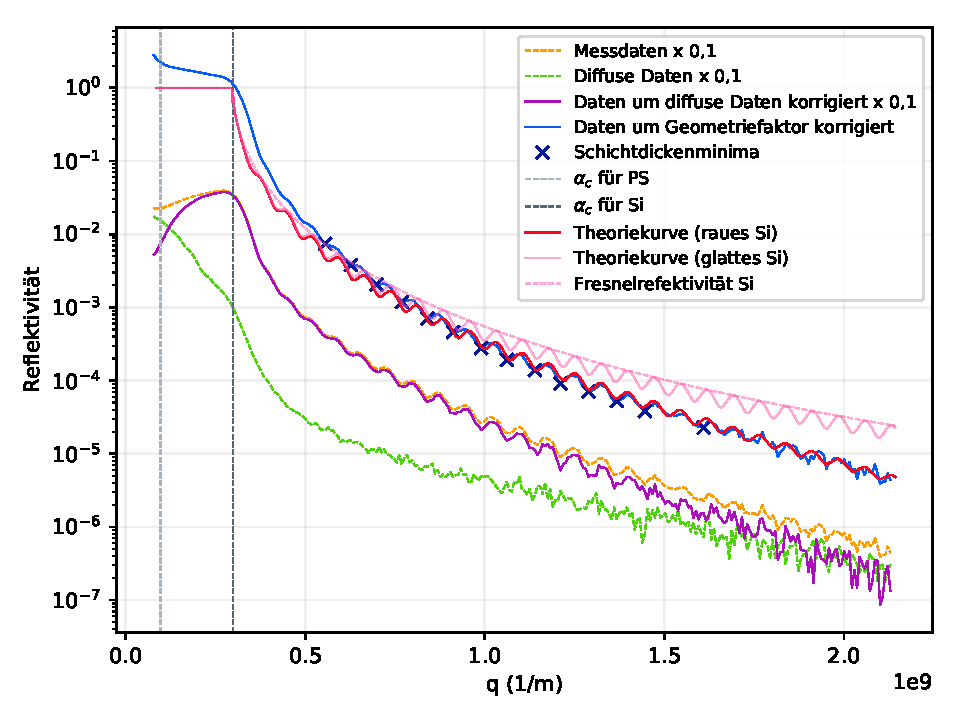
\includegraphics[scale=0.7]{content/plot4.pdf}
    \vspace{-10pt}
    \caption{Vermessungsdaten der Reflektivität PS-Si-Wafers in Abhängigkeit des Wellenvektorübertrages $q$.
            Zur Übersichtlichkeit sind einige Messdaten auf der logarithmischen Skala um 0,1 tiefer geschoben.}
    \label{fig:plot4}
\end{figure}

Schließlich werden zur Eliminierung von Rückstreueffekten im Schichtsystem, die Messdaten des Diffusen Scans
von den eigentlichen abgezogen.
Es erfolgt eine weitere Korrektur um den Geometriefaktor, welcher sich aus der Strahlbreite $d_0$ und dem 
Geometriewinkel $\alpha_g$ nach den Gleichungen \eqref{eqn:geome} bestimmen lässt. 
Diese verhindert die Unterrepräsentation sehr kleiner Winkel, für die nicht die gesamte Strahlbreite am Wafer 
reflektiert wird.\\

Anschließend werden die Positionen der Minima der Kiessig-Oszillationen mit Hilfe der Funktion
\textit{scipy.signal.find\_peaks} aus der Python-Bibliothek SkiPy bestimmt.
Aus deren Abständen kann die Schichtdicke des Polysterol(PS)-Films auf dem Silizium(Si)-Wafer bestimmt werden

\vspace{-20pt}
\begin{equation*}
    d_\text{PS} = (\num{882.43 +- 0.04}) \cdot 10^{-10} \si{\meter} \; .
\end{equation*}

Weiterhin wird mithilfe des Parrat-Algorithmus eine Theoriekurve an die 
korrigierten Messdaten durch Variation einiger Parameter gefittet.
Diese Parameter beinhalten Brechungsindizes $n$ der drei Materialien, 
die Rauigkeiten $\sigma$ der beiden Grenzflächen und die Schichtdicke $d_\text{PS}$.

\vspace{-35pt}
\begin{align*}
    n_\text{Luft} &= 1 \; ,\\
    n_\text{PS} &= 1 - \num{0.7e-6} \; ,\\
    n_\text{Si} &= 1 - \num{6.7e-6} \; ,\\
    \sigma_\text{Luft-PS} &= \SI{7.9e-10}{\meter} \; ,\\
    \sigma_\text{PS-Si} &= \SI{5.7e-10}{\meter} \; ,\\
    d_\text{PS} &= \SI{855e-10}{\meter} \; .
\end{align*}

Die kritischen Winkel der Totalreflexion der beiden Materialien
lassen sich aus den Korrekturen $\delta$ der Brechungsindizes 
$n = 1 - \delta$ berechnen zu

\vspace{-20pt}
\begin{align*}
    \alpha_\text{c,PS} &= \SI{0.068}{\degree} \; ,\\
    \alpha_\text{c,Si} &= \SI{0.210}{\degree} \; .\\
\end{align*}

\vspace{-20pt}
Zuletzt werden, durch den Parrat-Algorithmus berechnet, eine Theoriekurve der Reflektivität mit
ideal glatten Grenzflächen und die Fresnelreflektivität einer Siliziumoberfläche an der Luft eingezeichnet.

